\documentclass[a4paper,addpoints]{exam}

\usepackage[dvipsnames,table]{xcolor}
\usepackage{pgfplots}
\usetikzlibrary{decorations.markings}
\pgfplotsset{compat=1.8}
\usepackage{commath}
\usepackage{caption}
\usepackage{subcaption}
\usepackage{siunitx}
% russian integral
\usepackage{scalerel}
\DeclareMathOperator*{\rint}{\scalerel*{\rotatebox{17}{$\!\int\!$}}{\int}}
\qformat{\textbf{\large{Question \thequestion}}\hfill}
\pointsinrightmargin

\begin{document}

\begin{coverpages}

\begin{center}
  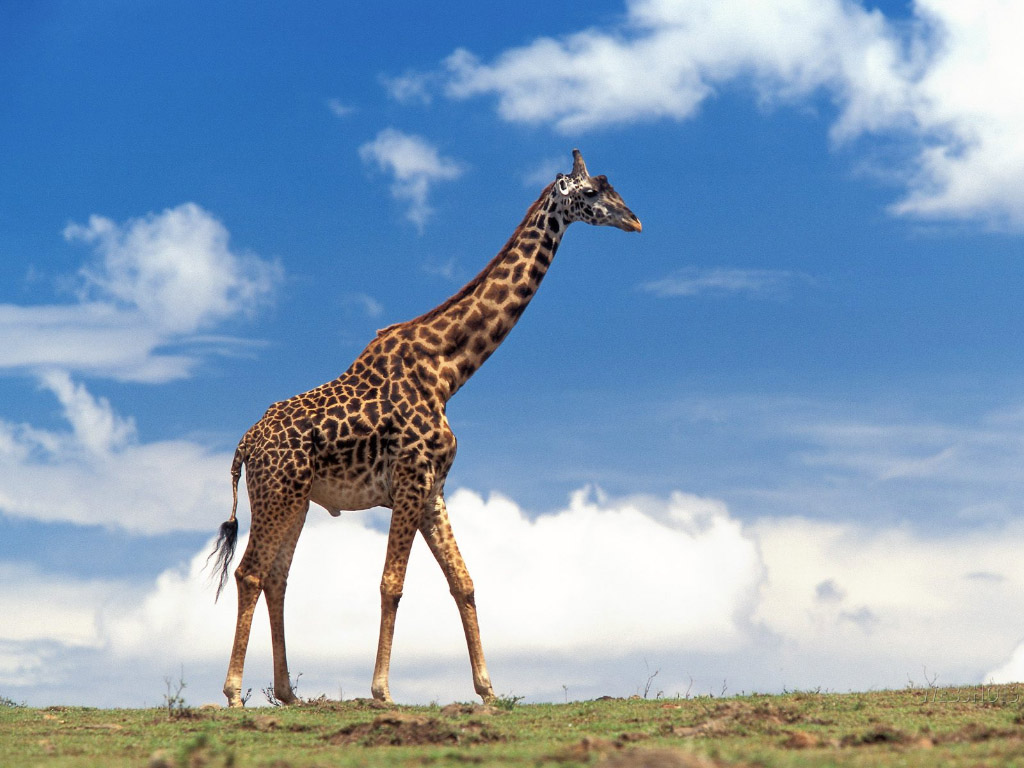
\includegraphics[width=0.4\textwidth]{giraffe}

  \vspace{5mm}

  \textbf{\Huge{Level One Mathematics\\Algebra}}
\end{center}

\vspace{5mm}

\noindent
\large{There are three questions, worth a total of \numpoints\ marks.\\
       Attempt ALL questions, showing all working.\\
       Read questions carefully before attempting them.\\
       Marks are available for partial answers.\\
       The amount of time expected to be spent per question may not necessarily correlate ``nicely'' to the number of marks.\\
       Diagrams may be used to support answers.\\
       Candidates who do not provide diagrams for some questions may be disadvantaged.\\
       Some marks are given for clarity and neatness of solutions or proofs.\\
       Excellence scripts must show evidence of relational thinking.\\
       Non-algebraic methods (e.g. ``guess-and-check'') will limit grades to an achieved.
       \vspace{2mm}

       \noindent CALCULATORS ARE NOT PERMITTED IN THIS EXAMINATION.}
\vspace{3mm}

\begin{tabular}{ll}
  \textbf{Time Allowed:}& One Hour\\
  \textbf{Achieved:}& 12 marks\\
  \textbf{Merit:}& 17 marks\\
  \textbf{Excellence:}& 21 marks
\end{tabular}

\vfill

\begin{center}
  \gradetable[h][questions]
  \vspace{2mm}

  \textbf{Available Grades:} \textit{Not Achieved}\quad\textit{Achieved}\quad\textit{Merit}\quad\textit{Excellence}
\end{center}

\end{coverpages}

\begin{questions}
  \question
    \begin{parts}
      \part[2] Consider the expression
            \begin{displaymath}
              \frac{xy^3 + x^2y}{x(y + 3x^2 y)} + 1.
            \end{displaymath}
        \begin{subparts}
          \subpart Simplify the expression as much as possible.
          \subpart What is the value of the expression when $ x = 1 $ and $ y = 2 $?
        \end{subparts}
      \part
        \begin{subparts}
          \subpart[3] The growth of a population of bacteria can be modelled, under certain assumptions, by an exponential equation
                   \begin{displaymath}
                     P(t) = A \cdot 3^{kt}.
                   \end{displaymath}
                   Suppose that the initial population of a particular colony of bacteria is 300 organisms, and that the population
                   triples after half an hour. Find the population after two hours.
          \subpart[3] Let $ Q(t) = B \cdot 2^{nt} $ and $ R(t) = (B + 1) 2^{nt} $. Suppose that $ 4Q(2) = R(2) $. Find $ B $ explicitly.
        \end{subparts}
    \end{parts}
  \question
    \begin{parts}
      \part[2] Find all the solutions of
            \begin{displaymath}
              (x^2 + 3x + 2)(3x^2 - 5x - 2) = 0.
            \end{displaymath}
      \part[3] Annie is three years older than Bridget. Nine years ago, Bridget's age was twice Annie's age. How old are Bridget
            and Annie today?
      \part[3] Charles has two fields. The second field is twice the size of the first. The smaller field has one side two kilometres
               longer than the other; the larger field is square, and has area \SI{48}{\kilo\metre\squared}.

               If the smaller field has area greater than \SI{4}{\kilo\metre\squared}, find its dimensions.
    \end{parts}
  \question
    \begin{parts}
      \part[1] Expand and simplify $ 3x(2x + 7y^2)y + 27y^3 + 5x(xy + 2yz) - (3xyz - 2x) $.
      \part[2] Suppose that
            \begin{displaymath}
              4x \leq -2x + 1
            \end{displaymath}
            and
            \begin{displaymath}
              2y < x + 3.
            \end{displaymath}
            Show that $ 4y < 7 $.
      \part[2] If $ x $ is even and $ y $ is odd, explain why $ x^2 + y + 1 $ cannot equal 3.
      \part[3] Bethany is trying to find all $ x $ that satisfy $ 6x^2 - x - 1 < 0 $; she follows the following steps.
            \begin{gather*}
              6x^2 - x - 1 = 0\\
              6x^2 + 2x - 3x - 1 = 0\\
              2x(3x + 1) - (3x + 1) = 0\\
              (2x - 1)(3x + 1) = 0\\
              \text{Since 6 is positive, the parabola opens upwards;}\\
              \text{so the parabola dips below the } x \text{ axis between these solutions.}\\
              2x - 1 = 0 \implies x = 1/2\\
              3x + 1 = 0 \implies x = -1/3\\
              \text{So the inequality is satisified when } -1/3 < x < 1/2.
            \end{gather*}
            Bert disagrees that her reasoning is correct: he doesn't think it makes sense to solve this inequality by solving
            the equation --- after all, the equation has just two solutions, while the solution to the inequality is an entire
            range of numbers.

            State who is correct, making sure to justify your answer with correct mathematical reasoning.
    \end{parts}
\end{questions}

\end{document}
